% !TEX encoding   = UTF8
% !TEX spellcheck = ru_RU

%%=================================
\chapter{Реализация и тестирование}
%%=================================

%%==========================================
\section{Особенности программной реализации}
%%==========================================

Структура кода расчётного модуля ZOOM DG выстроена таким образом, что для внедрения поддержки тетраэдральных элементов достаточно добавить правила преобразования и правила интегрирования. Идеи в коде представлены в виде типов. Так, например, идея кубатурных правил в коде выражена в виде типов \code{QRSide} и \code{QRCell}. А преобразование элементов представлено типами \code{ShapeFunctionSet2D} и \code{ShapeFunctionSet3D}. В виду существенных различий в вычислениях, связанных с объёмом, и в вычислениях, связанных с поверхностями, выделяются 2 иерархии классов: одна "--- для поверхностей, другая "--- для объёмов.



%%=========================
\subsection{Преобразования элементов} \label{subsect:2part:transform}
%%=========================

\begin{figure}[h]
	\centering
	\begin{tikzpicture}[nodes={font=\ttfamily\small, draw},
	rounded corners, level distance=10ex, >=Stealth]
	\graph [layered layout, components go right top aligned, edge=<-]
	{
		ShapeFunctionSet2D -> {
			QuadLinearElement[as=\tcol{QuadLinear\\Element}],
			QuadQuadraticElement[as=\tcol{QuadQuadratic\\Element}]
		};
		ShapeFunctionSet2D ->[blue] {
			TriLinearElement[blue, as=\tcol{TriLinear\\Element}],
			TriQuadraticElement[blue, as=\tcol{TriQuadratic\\Element}]
		};
	};
	\begin{scope}[on background layer]
	\node [draw, rounded corners,
	fit=(ShapeFunctionSet2D) (QuadLinearElement) (TriQuadraticElement)] {};
	\end{scope}
	\end{tikzpicture}
	\caption{Иерархия классов, реализующих преобразования граней}
	\label{pic:shapefunctions2d}
\end{figure}

\begin{figure}[h]
	\centering
	\begin{tikzpicture}[nodes={font=\ttfamily\small, draw},
	rounded corners, level distance=10ex, >=Stealth]
	\graph [layered layout, components go right top aligned, edge=<-]
	{
		ShapeFunctionSet3D -> {
			HexaLinearElement[as=\tcol{HexaLinear\\Element}],
			HexaQuadraticElement[as=\tcol{HexaQuadratic\\Element}]
		};
		ShapeFunctionSet3D ->[blue] {
			TetraLinearElement[blue, as=\tcol{TetraLinear\\Element}],
			TetraQuadraticElement[blue, as=\tcol{TetraQuadratic\\Element}]
		};
	};
	\begin{scope}[on background layer]
	\node [draw, rounded corners,
	fit=(ShapeFunctionSet3D) (HexaLinearElement) (TetraQuadraticElement)] {};
	\end{scope}
	\end{tikzpicture}
	\caption{Иерархия классов, реализующих преобразования элементов}
	\label{pic:shapefunctions3d}
\end{figure}

Ниже приведены фрагменты объявления базового класса преобразования поверхностных элементов~\ref{pic:shapefunctions2d}:

\begin{minted}[fontsize=\footnotesize, linenos]{C++}
class ShapeFunctionSet2D
{
protected:
  using ShapeFunc = std::function<QReal (QReal,QReal)>;

  vector<ShapeFunc> F;
  vector<ShapeFunc> dF_dXi, dF_dEta;

public:
  // ...

  zVec<QReal> transform (const vector<zVec<QReal>> &Xn,
                         QReal xi, QReal eta,
                         zVec<QReal> &N) const;
};
\end{minted}

\noindent
и фрагменты объявления базового класса преобразования объёмных элементов~\ref{pic:shapefunctions3d}:

\begin{minted}[fontsize=\footnotesize, linenos]{C++}
class ShapeFunctionSet3D
{
protected:
  using ShapeFunc = std::function<QReal (QReal,QReal,QReal)>;

  vector<ShapeFunc> F;
  vector<ShapeFunc> dF_dXi, dF_dEta, dF_dZeta;

public:
  // ...

  zVec<QReal> transform (const vector<zVec<QReal>> &Xn,
                         QReal xi, QReal eta, QReal zeta,
                         QReal &J) const;
};
\end{minted}

Базовые классы хранят набор функций формы и их производных и предоставляют метод \code{transform}, выполняющий преобразование в соответствии с соотношением~(\ref{eq:transform3d}) в трёхмерном случае и в соответствии с~(\ref{eq:transform2d}) в двумерном. Попутно производится вычисление элемента поверхности~\code{N} согласно формуле~(\ref{eq:normal}) и якобиана преобразования~\code{J}.

Конкретные наборы функций формы задаются при помощи производных классов. Например, ниже приведено объявление класса для задания <<линейного>> элемента поверхности тетраэдра:
\begin{minted}[fontsize=\footnotesize, linenos]{C++}
TriLinearElement::TriLinearElement ()
{
  // shape functions for corner nodes
  F.push_back ([](QReal xi, QReal eta) {return 1. - eta - xi;});
  F.push_back ([](QReal xi, QReal    ) {return xi;});
  F.push_back ([](QReal   , QReal eta) {return eta;});


  // derivative of shape functions with respect to xi
  dF_dXi.push_back ([](QReal, QReal) {return -1.;});
  dF_dXi.push_back ([](QReal, QReal) {return  1.;});
  dF_dXi.push_back ([](QReal, QReal) {return  0.;});


  // derivative of shape functions with respect to eta
  dF_dEta.push_back ([](QReal, QReal) {return -1.;});
  dF_dEta.push_back ([](QReal, QReal) {return  0.;});
  dF_dEta.push_back ([](QReal, QReal) {return  1.;});


  assert ( F      .size() == 3);
  assert (dF_dXi  .size() == 3);
  assert (dF_dEta .size() == 3);
}
\end{minted}

Функции формы и их производные располагаются в соответствующем векторе согласно нумерации узлов преобразования. В программе принята такая же нумерация, как и в Gmsh~\cite{Gmsh}. Таким образом, для преобразования тетраэдральных элементов необходимо было реализовать четыре класса, используя формулы (\ref{eq:tr:tetra:lin}) и (\ref{eq:tr:tetra:quad}). Двумерные преобразования получаются из трёхмерных, если добавить к ним дополнительное соотношение~(см.~подраздел~\ref{subsect:paramfaces}). Формулы для <<квадратичного>> элемента получаются довольно громоздкими, в них легко ошибиться. Был написан скрипт на \code{Python}~\cite{Python} с использованием библиотеки символьной математики \code{SymPy}~\cite{SymPy}, генерирующий фрагменты кода. Такой подход позволяет автоматизировать процесс и избавляет программиста от рутины, которая часто приводит к ошибкам.



%%=================================
\subsection{Правила интегрирования}
%%=================================

\begin{figure}[h]
	\centering
	\begin{tikzpicture}[nodes={font=\ttfamily\small, draw},
	                    rounded corners, level distance=5ex, >=Stealth]
	\graph [layered layout, components go right top aligned, edge=<-]
	{
		QRCell -> QRHexa -> {
			QRHexaOptimized,
			QRHexaGaLe
		};
		QRCell ->[blue] QRTetra[blue, text=blue]
		       ->[blue] QRTetraOptimized[blue, text=blue]
		       ->[blue] {
			QRTetraFirst[blue, as={QRTetra\_1\_1}],
			QRTetraJth[blue, as={...}],
			QRTetraNth[blue, as={QRTetra\_8\_43}]
		};
		QRTetra ->[blue, dashed] QRTetraGaLe[blue, dashed, text=blue, edge=dashed];
	};

	\begin{scope}[on background layer]
		\node [draw, rounded corners,
		       fit=(QRCell) (QRHexaOptimized) (QRTetraGaLe) (QRTetraNth)] {};
	\end{scope}
	\end{tikzpicture}
	\caption{Иерархия классов кубатурных правил интегрирования по объёму}
	\label{pic:cell:integrationrules}
\end{figure}

\begin{figure}[h]
	\centering
	\begin{tikzpicture}[nodes={font=\ttfamily\small, draw},
	                    rounded corners, level distance=5ex, >=Stealth]
	\graph [layered layout, components go right top aligned, edge=<-]
	{
		QRSide -> QRQuad -> {
			QRQuadOptimized,
			QRQuadGaLe
		};
		QRSide ->[blue] QRTri[blue, text=blue]
		       ->[blue] QRTriOptimized[blue, text=blue]
		       ->[blue] {
			QRTriFirst[blue, as={QRTri\_1\_1}],
			QRTriJth[blue, as={...}],
			QRTriNth[blue, as={QRTri\_13\_37}]
		};
		QRTri ->[blue, dashed] QRTriGaLe[blue, dashed, text=blue, edge=dashed];
	};

	\begin{scope}[on background layer]
	\node [draw, rounded corners,
	       fit=(QRSide) (QRQuadOptimized) (QRTriGaLe) (QRTriNth)] {};
	\end{scope}
	\end{tikzpicture}
	\caption{Иерархия классов кубатурных правил интегрирования по поверхности}
	\label{pic:side:integrationrules}
\end{figure}

Реализации двумерных и трёхмерных правил очень похожи, поэтому рассмотрим только двумерный случай. Базовый класс \code{QRSide} хранит координаты и веса квадратурных точек, а также для справочных целей максимальный порядок полинома, для которого формула абсолютно точна, и некий условный тип, несущий дополнительную информацию о квадратурном правиле (оптимальное, получено на основе одномерных квадратур Гаусса--Лежандра и т.\,п.). Интерфейс класса предоставляет небольшой набор методов, необходимых для работы: \code{size} "--- количество точек в формуле, \code{operator[]} "--- даёт доступ к координатам \code{i}-ой точки, \code{operator<} "--- определяет критерий упорядоченности (по увеличению вычислительной сложности, то есть количеству точек) правил во внешнем хранилище, и, наконец, методы \code{begin} и \code{end} обеспечивают поддержку конструкции языка \code{C++} <<\code{for-range}>>~\cite{Stroustrup:2013:en}. \code{is\_valid} "--- функция, проверяющая корректность кубатурной формулы, используя то свойство, что сумма всех кубатурных весов должна равняться объёму элемента. Так как у каждого элемента свой объём, эта функция является чисто виртуальной. Фрагменты класса приведены ниже:

\begin{minted}[fontsize=\footnotesize, linenos]{C++}
class QRSide : public z::Metadata
{
public:
  struct Point
  {
    QReal xi, eta;
    QReal weight;

    Point (QReal qxi, QReal qeta, QReal qweight)
      : xi {qxi}, eta {qeta}, weight {qweight}
    {}
  };

protected:
  std::vector<Point> points;

  virtual bool is_valid (size_t npoints, QReal eps) const = 0;

  // ...

public:
  const size_t order;
  const QRType type {QRType::Unknown};

  const Point & operator [] (size_t i) const;

  bool operator < (const QRSide& rhs) const;

  size_t size () const  {return points.size();}

  std::vector<Point>::const_iterator begin () const;
  std::vector<Point>::const_iterator end   () const;
};
\end{minted}

\noindent
Объявление класса \code{QRTetra} выглядит следующим образом:

\begin{minted}[fontsize=\footnotesize, linenos]{C++}
class QRTetra : public QRCell
{
protected:
  using QRCell::QRCell;  // inherits constructors

  bool is_valid (size_t npoints, QReal eps) const override;

public:
  ~QRTetra () override = 0;
};
\end{minted}

В данной работе использовались оптимизированные симметричные кубатурные правила~\cite{CubatureRules}, позволяющие интегрировать полиномы по тетраэдрам до 8-й степени и по треугольникам до 13-й степени. Под \textit{симметричными кубатурными правилами} (Fully Symmetric) подразумевается следующее: если кубатурное правило содержит точку \(\{L_1, L_2, L_3, L_4\}\) с весом~\(\alpha\), то оно также содержит и точку \(\{L_{p_1}, L_{p_2}, L_{p_3}, L_{p_4}\}\) с весом~\(\alpha\), где \(\{p_1, p_2, p_3, p_4\}\) "--- любая перестановка \(\{1, 2, 3, 4\}\). Если все \(L_i\) различны, то мы получим \(4! = 24\) кубатурных точек. В дальнейшем возможно добавление кубатурных правил произвольного порядка на основе квадратур Гаусса, см.~подраздел~\ref{subsect:tetrarules}.

Все оптимизированные квадратурные правила наследуют от класса \code{QRTriOptimized}:

\begin{minted}[fontsize=\footnotesize, linenos]{C++}
class QRTriOptimized : public QRTri
{
protected:
  void addFullySymmetric (QReal a, QReal b, QReal w);

  QRTriOptimized (size_t maxorder, QRType qrtype = QRType::Optimized)
    : QRTri {maxorder, qrtype}
  {}

public:
  ~QRTriOptimized () override = 0;
};
\end{minted}

Сложность реализации этого класса в трёхмерном случае заключалась в написании функции \code{addFullySymmetric}: требовалось рассмотреть 15 вариантов расположения кубатурной точки в тетраэдре, в последнем из которых необходимо было добавить 24 кубатурные точки. Для реализации функции, используя язык \code{Python}, был осуществлен перебор всех возможных вариантов и написан генератор исходного текста.

Ниже приведён пример класса, который реализует конкретную квадратурную формулу, состоящую из 4-х точек и точную для полиномов степени не выше 3-й:

\begin{minted}[fontsize=\footnotesize, linenos]{C++}
class QRTri_3_4 : public QRTriOptimized
{
public:
  QRTri_3_4 ();
};
\end{minted}

Как и в случае реализации правил преобразования элементов (см. подраздел~\ref{subsect:2part:transform}), основную работу по заполнению массива точек выполняет конструктор класса:

\begin{minted}[fontsize=\footnotesize, linenos]{C++}
QRTri_3_4::QRTri_3_4 ()
  : QRTriOptimized {3}
{
  QReal a = 0., b = 0., w = 0.;

  a = 0.333333333333333333333333333333333L;
  b = 0.333333333333333333333333333333333L;
  w = -0.28125L;
  addFullySymmetric (a, b, w);

  a = 0.2L;
  b = 0.2L;
  w = 0.260416666666666666666666666666666L;
  addFullySymmetric (a, b, w);

  assert (is_valid (4));
}
\end{minted}



%%====================
\section{Тестирование}
%%====================

%%===========================================
\subsection{Математическая постановка задачи}
%%===========================================

В качестве тестовой задачи рассматривается обтекание цилиндра невязким сжимаемым дозвуковым потоком. Характерная картина течения представлена на рис.~\ref{pic:result:mach}.

\begin{figure}[ht]
	\centering
	\includegraphics[width=1.\textwidth]{cylinder_tetra_fine_K3_Mach}
	\caption{Характерная картина течения при обтекании цилиндра. Показаны поле числа Маха, расчётная сетка и линии тока}
	\label{pic:result:mach}
\end{figure}

Обтекание цилиндра выбрано по следующим причинам: задача простая, а решение задачи экспериментально и теоретически изучено, см.~\cite{CylynderFlow:1994:en}. Обтекаемое тело имеет криволинейную форму, что позволяет протестировать преобразования координат и выяснить, как они влияют на ошибку в решении. Для выполнения расчёта необходимо построить расчётную сетку, а также задать начальные и граничные условия.

Сперва для знакомства с программой была построена расчётная сетка, состоящая из гексаэдральных элементов. Затем для тестирования была построена сетка из тетраэдральных элементов. Сетка строилась с использованием трёхмерного генератора конечно-элементных сеток Gmsh~\cite{Gmsh}.

Характеристики расчётной области: высота цилиндра равна 100 м, радиус цилиндра 1 м, внешняя граница расчётной области удалена от центра цилиндра на 1000 м. Для уменьшения флуктуаций вдоль оси цилиндра использовалась всего одна ячейка. Характеристический размер вдоль азимута равномерный, вдоль радиуса "--- подчиняется геометрической прогрессии.

\begin{figure}[h]
	\centering
	\includegraphics[width=0.8\textwidth]{hexa_mesh}
	\caption{Гексаэдральная расчётная сетка}
	\label{pic:hexamesh}
\end{figure}

\begin{figure}[h]
	\centering
	\includegraphics[width=0.8\textwidth]{tetra_mesh}
	\caption{Тетраэдральная расчётная сетка}
	\label{pic:tetramesh}
\end{figure}

Так как задача стационарная, а решение симметрично в верхней и нижней полуплоскостях, то сетка строилась только для половины расчётной области цилиндра. В плоскости симметрии используются симметричные граничные условия, на поверхности цилиндра твёрдая стенка без прилипания, а на внешней границе области "--- условие свободного вытекания.

В качестве начального условия было задано равномерное поле с параметрами, как в набегающем потоке: давление \(p_\infty = 100\,000\) Па, плотность \(\rho_\infty = 1.19\) кг/\(\text{м}^3\), скорость, направленная поперёк цилиндра, \(u_\infty = 50\) м/с, остальные компоненты скорости равны нулю.

Пример гексаэдральной и тетраэдральной расчётных сеток показан на рис.~\ref{pic:hexamesh} и рис.~\ref{pic:tetramesh}.



%%==================================
\subsection{Результаты тестирования}
%%==================================

Расчёты проводились с различными степенями базисных полиномов \(K~=~0, 1, 2, 3, 4\) для двух видов сеток: с <<линейными>> и <<квадратичными>> элементами. Характеристики расчётной сетки в обоих случаях одинаковы (см.~рис.~\ref{pic:tetramesh}): количество ячеек у цилиндра равно 3, коэффициент прогрессии равен 2. Сетка получилась довольно грубой: количество тетраэдров равно 315.

Известно, что сопротивление цилиндра в случае невязкого обтекания равно нулю, а поле полного давления равномерно во всем пространстве. По этим параметрам можно оценить ошибку.

\begin{figure}[ht]
	\centering
	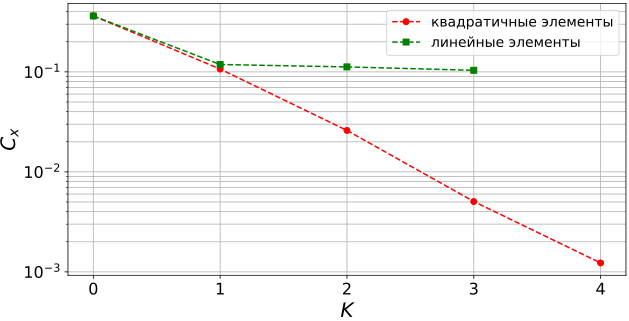
\includegraphics[width=0.8\textwidth]{Cx}
	\caption{Убывание ошибки в определении коэффициента сопротивления \(C_{x}\) в зависимости от порядка базисных функций \(K\)}
	\label{pic:Cx}
\end{figure}

На рис.~\ref{pic:Cx} показано убывание логарифма ошибки определения коэффициента сопротивления в зависимости от порядка базисных функций. Видно, что для \(K = 0\) и \(K = 1\) ошибки у <<квадратичных>> и <<линейных>> тетраэдров идентичны. Но с дальнейшим увеличением \(K\) ошибка в случае <<линейных>> элементов практически не убывает. Для расчёта на сетке с <<линейными>> элементами с \(K = 3\) пришлось сильно уменьшить шаг по времени, иначе метод не сходился. Из графика видно, что использование <<квадратичных>> элементов при \(K \geq 2\) позволяет уменьшить ошибку при вычислении сопротивления цилиндра на несколько порядков.

\begin{figure}[ht]
	\centering
	\includegraphics[width=0.7\textwidth]{K2_quad}
	\caption{Поле полного давления, \(K = 2\), <<квадратичные>> тетраэдры. Нечёткость картины связана с грубой визуализацией}
	\label{pic:p_stagnation}
\end{figure}

Рассмотрим теперь картину полного давления для разных порядков базисных функций \(K\). Полное давление вычисляется по следующей формуле: 
\[p_{0\infty} = p_\infty \left(1 + \frac{\gamma-1}{2}M_{\infty}^2\right)^\frac{\gamma}{\gamma - 1},\] 
где \(\gamma\) "--- показатель адиабаты, \(M\) "--- число Маха. Из рис.~\ref{pic:p_stagnation} видно, что за цилиндром возникает область падения поля полного давления. Рассмотрим точку \(\mathbf x_b\), расположенную сразу за цилиндром: \(x_b = 1\) м, \(y_b = 0\) м. Можно попытаться определить ошибку, вычислив \(\left|\Delta p_0\right| = \left|p_{0\infty} - p_0(\mathbf x_b)\right|\). На рис.~\ref{pic:p_error} показано убывание ошибки в зависимости от степени базисных функций в точке~\(\mathbf x_b\). Картина аналогична тому, что мы видели на рис.~\ref{pic:Cx}: при \(K = 0\) и \(K = 1\) ошибки идентичны, а при увеличении порядка~\(K\) ошибка в случае <<квадратичных>> элементов уменьшается больше, чем в случае <<линейных>>.

\begin{figure}[ht]
	\centering
	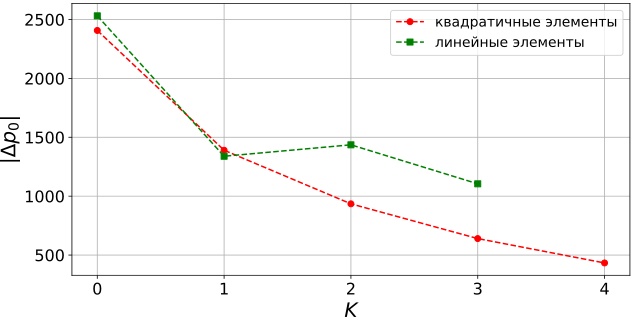
\includegraphics[width=0.8\textwidth]{p0}
	\caption{Убывание ошибки полного давления \(p_{0}\) в точке за цилиндром в зависимости от порядка базисных функций \(K\)}
	\label{pic:p_error}
\end{figure}

На рис.~\ref{pic:result:mach} показан результат единичного расчёта на подробной сетке. Количество рёбер у цилиндра равно 32, коэффициент геометрической прогрессии равен~\(1.075\). В качестве базисных функций были взяты полиномы 3 степени. К завершению расчёта в задаче прошло 50 секунд физического времени. Вычисления длились почти 5 суток на Core i7 Haswell. Общее количество тетраэдров составило 26436.